\documentclass[12pt]{article}

\title{SAMx8: Dragon 64 512K expansion}
\author{Ciaran Anscomb \textit{<www@6809.org.uk>}}
\date{}

\usepackage[a4paper,margin=1in]{geometry}

\usepackage[utf8]{inputenc}
\DeclareUnicodeCharacter{00A0}{~}

\pretolerance=7500
\tolerance=2000
\emergencystretch=12pt

\usepackage{graphicx, float, rotating}
\usepackage[hidelinks]{hyperref}

\usepackage[T1]{fontenc}  % T1 fonts, please
\usepackage{nimbusmono}
\usepackage{nimbusserif}

\makeatletter
\newcommand*{\textoverline}[1]{$\overline{\hbox{#1}}\m@th$}
\makeatother

\newenvironment{compactlist}
{ \begin{itemize}
  \setlength{\itemsep}{0pt}
  \setlength{\parskip}{0pt}
  \setlength{\parsep}{0pt} }
{ \end{itemize} }


\begin{document}

\maketitle

The SAMx8 is a 512K SRAM expansion and MMU for the Dragon 64.  It enables
arbitrary mapping of 16K pages in two tasks, optionally making either or both
of the top two 4K regions common to all memory maps.

The speed of modern SRAM allows the SAMx8 to include a RAM access cycle for
video data even in the FAST CPU rate setting.  Additionally, the video base
address can be set to any multiple of 32 bytes across the entire 512K.

There are some trade-offs:  The register that selected address-dependent CPU
rate now simply duplicates selection of fast mode.  Support for undocumented
video address ``glitching'' is removed in favour of the finer-grained video
address control.  Also, any feature that was only there to support DRAM has
been removed.


\subsection*{Fitting}

\textbf{Warning:} Fitting this board requires a modification to the original
motherboard.  Although the Dragon 64 PCB is pretty robust, this is old
hardware, so I do not recommend trying this if you're not confident in your
desoldering skills.  Lifted pads or tracks may ensue.

To install, first desolder IC25 (74LS244) and fit a 20 pin DIP socket in its
place.  Remove the SAM from its socket (IC39).  The expansion is designed to
plug into both of these sockets, replacing the function of both ICs.

The curious shape of the expansion (see Figure~\ref{fig:pcb}) fits it around
two other ICs on the motherboard, in case these are also socketed, e.g. if
you've hand-built a Dragon 64 reproduction motherboard.  The expansion is
designed such that memory on the motherboard is never selected, so if your DRAM
ICs are soldered in that's fine; however, if they're socketed and you're able
to remove them, you'll save a little bit of power.

\begin{figure}
	\centering
	\setlength{\belowcaptionskip}{10pt plus 3pt minus 2pt}
	\caption{SAMx8 PCB}
	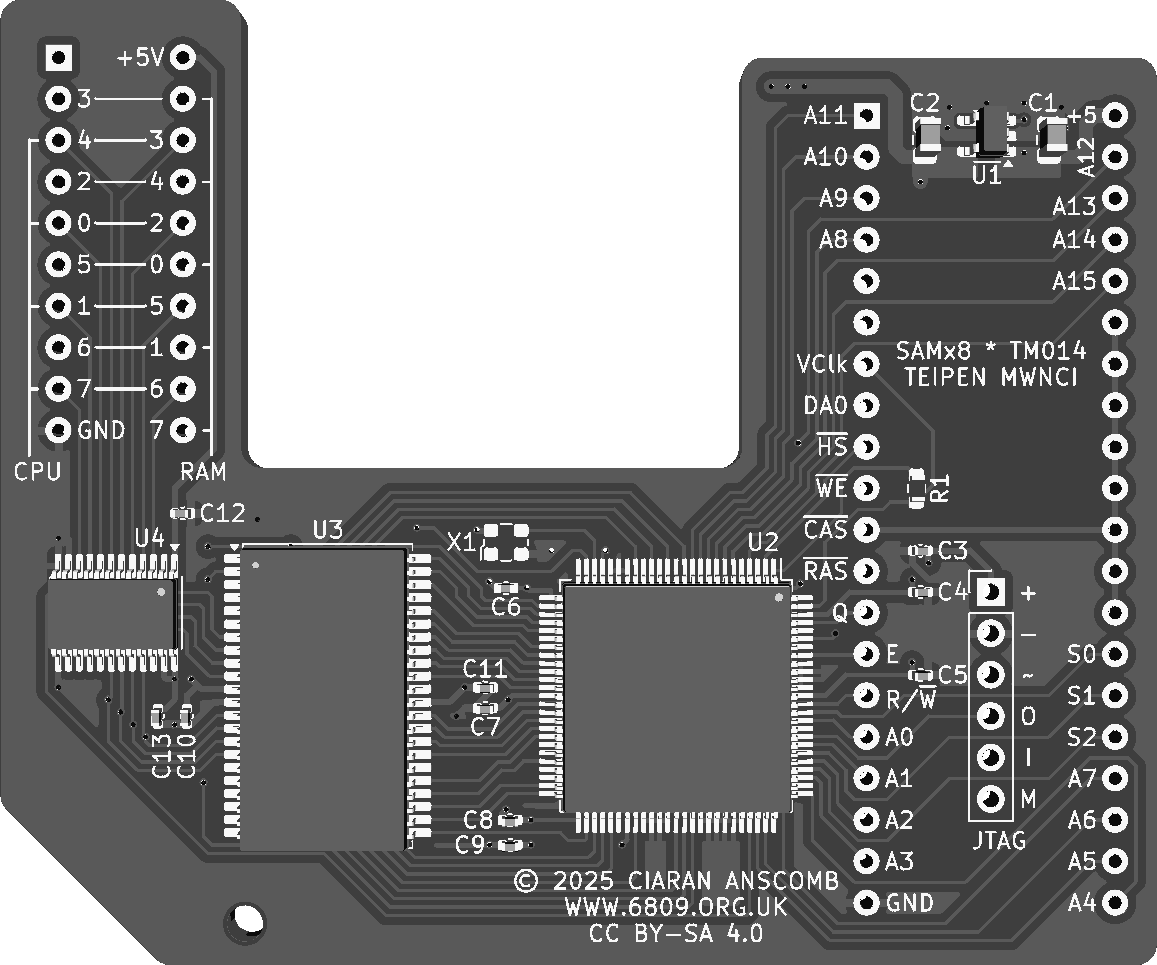
\includegraphics[width=0.40\linewidth]{samx8-pcb.png}
	\label{fig:pcb}
\end{figure}


\subsection*{Programming guide}

Most of the SAM's registers remain for compatibility.  Bits are cleared by
writing to \textit{even} addresses, and set by writing to \textit{odd}
addresses, and have the following purposes:

\begin{table}[H]
\small
\centering
\setlength\tabcolsep{4pt}
\begin{tabular}{llll}
Address & Function & Address & Function \\ \hline\rule{0pt}{2.6ex}\rule[-0.9ex]{0pt}{0pt}%
\$FFC0 & V0 clear & \$FFC1 & V0 set \\
\$FFC2 & V1 clear & \$FFC3 & V1 set \\
\$FFC4 & V2 clear & \$FFC5 & V2 set \\
\$FFC6 & F9 clear & \$FFC7 & F9 set \\
\$FFC8 & F10 clear & \$FFC9 & F10 set \\
\$FFCA & F11 clear & \$FFCB & F11 set \\
\$FFCC & F12 clear & \$FFCD & F12 set \\
\$FFCE & F13 clear & \$FFCF & F13 set \\
\$FFD0 & F14 clear & \$FFD1 & F14 set \\
\$FFD2 & F15 clear & \$FFD3 & F15 set \\
\$FFD4 & TASK 0 & \$FFD5 & TASK 1 \\
\$FFD6 & SLOW CPU & \$FFD7 & FAST CPU \\
\$FFD8 & SLOW CPU & \$FFD9 & FAST CPU \\
\$FFDA & - & \$FFDB & - \\
\$FFDC & - & \$FFDD & - \\
\$FFDE & 32K RAM / 32K ROM & \$FFDF & 64K RAM
\end{tabular}
\end{table}

V0--V2 selects VDG mode in the same way as the SAM.

F9--F15 have been renamed here to better reflect their function: you are
clearing or setting the numbered bit within the video base address register.

The ``page'' bit in the SAM (\$FFD4/5) has been repurposed as a TASK select
register.  The default page mapping on reset for TASK 1 provides similar
behaviour to the old page bit.

Address-dependent CPU rate has been removed, so the bits at \$FFD6/7 switch
between slow and fast mode in the same way as \$FFD8/9.

New registers provide access to the extra RAM.  For these registers, the value
on the data bus is used, though they remain \textit{write-only}.  The default
values shown are initialised on power on and reset.

\begin{table}[H]
\small
\centering
\setlength\tabcolsep{4pt}
\begin{tabular}{lll}
Address & Function & Default \\ \hline\rule{0pt}{2.6ex}\rule[-0.9ex]{0pt}{0pt}%
\$FF30 & Page in TASK 0 mapped to \$0000--\$3FFF & 0 \\
\$FF31 & Page in TASK 0 mapped to \$4000--\$7FFF & 1 \\
\$FF32 & Page in TASK 0 mapped to \$8000--\$BFFF & 2 \\
\$FF33 & Page in TASK 0 mapped to \$C000--\$FEFF & 3 \\
\$FF34 & Page in TASK 1 mapped to \$0000--\$3FFF & 2 \\
\$FF35 & Page in TASK 1 mapped to \$4000--\$7FFF & 3 \\
\$FF36 & Page in TASK 1 mapped to \$8000--\$BFFF & 2 \\
\$FF37 & Page in TASK 1 mapped to \$C000--\$FEFF & 3 \\
\$FF38 & F13--F18 (6 bits of video RAM base) & 0 \\
\$FF39 & F5--F12 (8 bits of video RAM base) & 0 \\
\$FF3F & COMMON (2 bits) & 0
\end{tabular}
\end{table}

Each of the eight mapping registers (four each for two tasks) accepts a 5-bit
page number (0--31), mapping an arbitrary 16K page of SRAM to that region of
the CPU's address space.

Setting bit 0 of COMMON forces the top 4K (\$F000--\$FEFF and the vector area
\$FFE0--\$FFFF) to be mapped to page 31 whatever other configuration is in
place.  Setting bit 1 does the same for the next 4K down (\$E000--\$EFFF).  The
vector area is still read-only, and in map type 0 so is the rest, however
modifications can be made by mapping page 31 elsewhere.  An example use of this
function is to have a small ``kernel'' handling interrupt dispatch consistently
even as tasks are switched or memory is remapped.

Writes to \$FF38/9 allow you to set multiple bits of the video RAM base
register at once.  They also expose extra high bits to locate video RAM
anywhere within the 512K, and extra low bits to allow it to start at any
multiple of 32 bytes.


\subsection*{Timing}

One machine cycle comprises 16 cycles of the on-board oscillator (T0--TF),
during which there is a video RAM fetch and one or two CPU cycles (depending on
configured CPU rate).  Most operation is synchronous with the oscillator, but
changes in A13--A15 are immediately reflected in S0--S2.

The MC6809E datasheet documents the ``Address Delay Time''
(t\textsubscript{AD}) in the BUS TIMING CHARACTERISTICS table.  This tells us
that the next address from the CPU should be available 3 (2.8) oscillator
periods after E falls during a slow cycle or 2 (1.44) periods during a fast
cycle.  Transition points between SLOW and FAST mode should be chosen with
care:

In a SLOW cycle (see Figure~\ref{fig:slowcycle}), video memory access is
between T1 and T3, with \textoverline{RAS0} rising at T2 to latch the data.
CPU memory access is between TC and TF.  Any decision to transition to FAST
cycles is taken at TC, which results in truncating E by one cycle.

In a FAST cycle (see Figure~\ref{fig:fastcycle}), video memory access is
between TF and T1, with \textoverline{RAS0} rising at T0 to latch the data.
CPU memory accesses are between T4 and T6, and between TC and TE.  Decisions to
transition from FAST to SLOW are taken at T0 and T8.

If a DA0 transition occurs outside the window TA--TC, VClk is stopped until TB
to resynchronise the VDG.

\begin{sidewaysfigure}
	\centering
	\setlength{\belowcaptionskip}{10pt plus 3pt minus 2pt}
	\caption{Timing waveforms for CPU RATE = SLOW}
	\includegraphics[width=\linewidth]{samx8-slow-timing.png}
	\label{fig:slowcycle}
\end{sidewaysfigure}

\begin{sidewaysfigure}
	\centering
	\setlength{\belowcaptionskip}{10pt plus 3pt minus 2pt}
	\caption{Timing waveforms for CPU RATE = FAST}
	\includegraphics[width=\linewidth]{samx8-fast-timing.png}
	\label{fig:fastcycle}
\end{sidewaysfigure}


\newpage
\subsection*{CPLD design}

The SAMx4 replaced the entire functionality of the SAM with an XC95144XL CPLD
and minimal interfacing.  Although the obvious next step is to use this code in
a larger device and add more features, I decided to explore what could be
achieved in the same space if we assume we also want to switch to using
available fast SRAM.

Because the memory is specified, a lot of the complexity for handling different
RAM sizes can be stripped out.  Similarly, because it's SRAM, no refresh is
required.

And because SRAM is \textit{fast}, I looked into whether there was enough
room in the SAM timing to squeeze in a video fetch even in fast CPU rate.
There is, so given we can now run double speed all the time\footnote{If you
plan to run double speed, you should also ensure that your CPU and PIA ICs are
replaced with suitably rated parts.}, I decided to take a leaf out of the CoCo 3
GIME's book and not support address-dependent mode at all, saving some more
space.

The SAMx4 goes to lengths to reproduce known but undocumented video address
``glitching''.  This is also quite expensive in terms of CPLD space, so for
this experiment, out it goes.

Dropping these features frees up enough space for the page registers, COMMON
flags and more fine-grained video RAM base control.


\subsection*{Physical design}

To interface SRAM to the motherboard, we need data to be presented to the video
latch and to buffer it to or from the CPU.  IC25 has all of these lines
available, and is relatively close to the SAM physically, so putting a socket
here seems like the logical choice.

The board is laid out such that all SMT components are on the top side; you can
use a PCB manufacturer's single-side SMT assembly service and just attach the
board-to-board connectors yourself.

The main parts are:

\begin{itemize} \item Xilinx XC95144XL CPLD.  Programmed to provide both SAM
functionality, and extra control lines to the rest of the board.

\item ISSI IS61WV25616BLL-10TI SRAM.  This is actually organised as 256K × 16 bits.
Chosen purely due to availability.

\item Nexperia 74LVC4245A-Q100 Octal dual supply translating transceiver.
\end{itemize}

The ``translating transceiver'' acts as a bidirectional buffer between the CPU
data bus and the SRAM, and has a tri-state control to isolate it when not in
use by the CPU.  It also provides level translation between the 5V TTL CPU and
the 3.3V CMOS SRAM.  Although the Xilinx CPLD has 5V tolerant inputs, the
selected SRAM IC does not, so this is required.  The video latch is input-only,
so for that, the 3.3V SRAM lines can be connected directly (3.3V CMOS as output
is compatible with 5V TTL as input).

As a side note, if you look to employ level shifting yourself, remember that 5V
CMOS has very different characteristics to 5V TTL; the Nexperia part explicitly
documents TTL compatibility, other seemingly similar chips may not.

The chosen SRAM IC is 16-bit, but provides separate lower and upper byte
control lines (\textoverline{LB} and \textoverline{UB}), with unselected bytes
being excluded from writes, and going high impedance on reads.  To work in an
8-bit system, we simply connect lines from the upper and lower bytes together
and only select one byte at a time.  It is probably quite important that the
chip is not enabled (\textoverline{CE} low) until the outputs to
\textoverline{LB} and \textoverline{UB} are stable, else there may be brief
high-current periods between the two halves.

The connections to the motherboard are into IC sockets, and for the
board-to-board connectors I would steer clear of the ``standard'' pin header
strips.  They tend to have 0.64mm square pins, and these can be (way) too large
for a socket.  Instead, I recommend connectors with machined pins, preferably
with 0.64mm diameter for soldering to the PCB, and 0.5mm diameter on the other
side for inserting into the sockets.

I've used CnC Tech 220-1-XX-00X male-to-male DIL headers, and they work very
well.  Unfortunately, these had to be ordered from the USA; I could find no
similar product listed by the usual UK distributors.

Previously, I've used Samtec TS-1XX-T-A (or -G-A) pin headers.  As single-row
strips, you need to be a little more careful that things stay lined up while
soldering, but they also fit well.  However, they seem to be \textit{very}
expensive, and end up being a significant fraction of the cost of the BOM.

Whichever you choose, solder the connectors to the underside of the board
(components facing upwards).


\subsection*{Further development}

Well, aside from bug fixes, probably none.  That is, the SAMx8 is an experiment
to see what useful functionality can be squeezed into the specific 144-macrocell
CPLD used in the SAMx4.

That said, here are some possible considerations that a larger CPLD would
enable without much more in the way of development:

\begin{itemize}
\item Finer grained pages and/or
\item more tasks and/or
\item more RAM.
\item Additional fine-grained video RAM offset of 0--31.
\end{itemize}

All those page bits multiply up, however, so the real next step is probably to
offload all the page mapping registers into more external SRAM, addressed by
TASK register and however many address bits from the CPLD.  As power-up
initialisation of that SRAM could be tricky, you'd probably want to be
bypassing that mapping by default.  You could encode extra features (e.g.
write-protect flags) into each page select this way.

Whether I look into this myself really does depend on whether I ever feel the
pinch of only having a ``mere'' 512K.


\newpage
\subsection*{Similar products}

Stewart Orchard produced a 256K ``banker board'', allowing less arbitrary
mappings of 32K blocks within 256K of DRAM (which can be installed in place of
the 4164s on the existing motherboard, so long as care is taken to isolate and
separately link their extra address line).  The SAMx4 reproduced this scheme.
\href{https://gitlab.com/sorchard001/dragon-256k-banker-board}{https://gitlab.com/sorchard001/dragon-256k-banker-board}

The MOOH is a cartridge expansion by Tormod Volden.  It provides finer-grained
page mapping and even an SD card interface.  However, because it is a
cartridge, it has no ability to affect video RAM operation, so writes to the
on-board RAM are passed through for video data.
\href{http://tormod.me/mooh.html}{http://tormod.me/mooh.html}

Julian Brown has various plans for new Dragon motherboards, expanding
capabilities in more ways than just memory.  Watch this space:
\href{https://github.com/jimbro1000}{https://github.com/jimbro1000}

The in-development CoCoMEM Jr. looks like it is intended to work with extra
external SRAM as described above.  It is presented as interposing the CPU
rather than the SAM, and I'm not sure how it's intended to interface to video
data---possibly it will pass writes through to main RAM like the MOOH.
\href{http://www.go4retro.com/products/cocomem-jr/}{http://www.go4retro.com/products/cocomem-jr/}


\subsection*{License}

Released under the Creative Commons Attribution-ShareAlike 4.0 International
(CC BY-SA 4.0).  Full text in the \texttt{LICENSE} file.

You are free to:

\begin{itemize}
\item \textbf{Share} --- copy and redistribute the material in any medium or
format
\item \textbf{Adapt} --- remix, transform, and build upon the material for any purpose,
even commercially.
\end{itemize}

The licensor cannot revoke these freedoms as long as you follow the license terms.

Under the following terms:

\begin{itemize}
\item \textbf{Attribution} --- You must give appropriate credit, provide a link to the license, and indicate if changes were made. You may do so in any reasonable manner, but not in any way that suggests the licensor endorses you or your use.

\item \textbf{ShareAlike} --- If you remix, transform, or build upon the material, you must distribute your contributions under the same license as the original.
\end{itemize}

\textbf{No additional restrictions} --- You may not apply legal terms or technological measures that legally restrict others from doing anything the license permits.


\subsection*{Revision history}

\textbf{2025-04-25} Minor changes in phrasing for version 1.0.\\
\textbf{2025-04-19} Various functionality and timing changes since the release candidates.


\end{document}
